\documentclass[11pt,a4paper]{article}

\usepackage[T1]{fontenc}
\usepackage[utf8]{inputenc}
\usepackage{lmodern}
\usepackage{geometry}
\usepackage{graphicx}
\usepackage{booktabs}
\usepackage{enumitem}
\usepackage{hyperref}
\usepackage{titlesec}
\usepackage{parskip}
\usepackage{caption}

\geometry{margin=2.1cm}
\setlist[itemize]{leftmargin=1.3em,itemsep=0.2em}
\hypersetup{colorlinks=true,linkcolor=black,urlcolor=blue}
\captionsetup{font=small,skip=4pt}
\titleformat{\section}{\large\bfseries}{\thesection}{0.6em}{}
\titlespacing*{\section}{0pt}{1.1em}{0.4em}

\title{\textbf{Sentinel-1 / Sentinel-2 land-cover classification of Porto}\\[0.35em]
\large SNAP collocation, Random Forest, and why 100\% accuracy is not a result}
\author{Aleksandra Pacia \quad Erasmus, Geospatial Engineering, Universidade do Porto\\
{\small Home university: AGH Krakow \quad Supervisor meeting note, 26 October 2026}}
\date{}

\begin{document}
\maketitle
\vspace{-1.4em}

\noindent\textit{This note summarises work already done in SNAP and Python. It is not a claim of operational land-cover mapping. Repository: \url{https://github.com/aleksandrapacia/PortoProject}.}

\section{Aim}
To test whether collocated \textbf{Sentinel-1 SAR} and \textbf{Sentinel-2 optical} data, processed in SNAP and classified in Python, can separate four land-cover classes over Porto and the Douro valley: water, vegetation, urban, bare soil --- and to treat accuracy numbers as something to \textbf{audit}, not to advertise.

\section{Method (what was actually run)}
\begin{itemize}
  \item \textbf{SNAP:} collocation of Sentinel-1 GRD ($\sigma^0$ VV, VH) with Sentinel-2; MNDWI and NDVI computed as auxiliary layers.
  \item \textbf{Labels (v1):} pixel thresholds on MNDWI, NDVI and VH (water / vegetation / urban / soil). These are \emph{not} independent ground truth.
  \item \textbf{Classifier:} Random Forest on \textbf{raw} bands only --- B2, B3, B8, B11, $\sigma^0$ VV, $\sigma^0$ VH. Indices were kept out of the feature vector after a 100\% score showed leakage.
  \item \textbf{Validation:} stratified random split \emph{and} spatial block cross-validation (\texttt{GroupKFold} on a $10\times10$ grid).
\end{itemize}

\section{Results}
A random split produced essentially perfect scores (water and vegetation $F_1 = 1.00$; urban $\approx 0.97$; overall accuracy $\approx 1.00$). Spatial-block CV stayed near $0.99$. That is still too high to believe as map accuracy: the labels remain threshold rules on the same image.

What \emph{is} usable: the classified map is spatially coherent (ocean and Douro as water; built-up as fragmented red; vegetation dominant inland), and feature importance shows NDVI-related optical structure as the main driver, with \textbf{VH backscatter} contributing to the urban class --- i.e.\ radar is not redundant.

\begin{figure}[h]
\centering
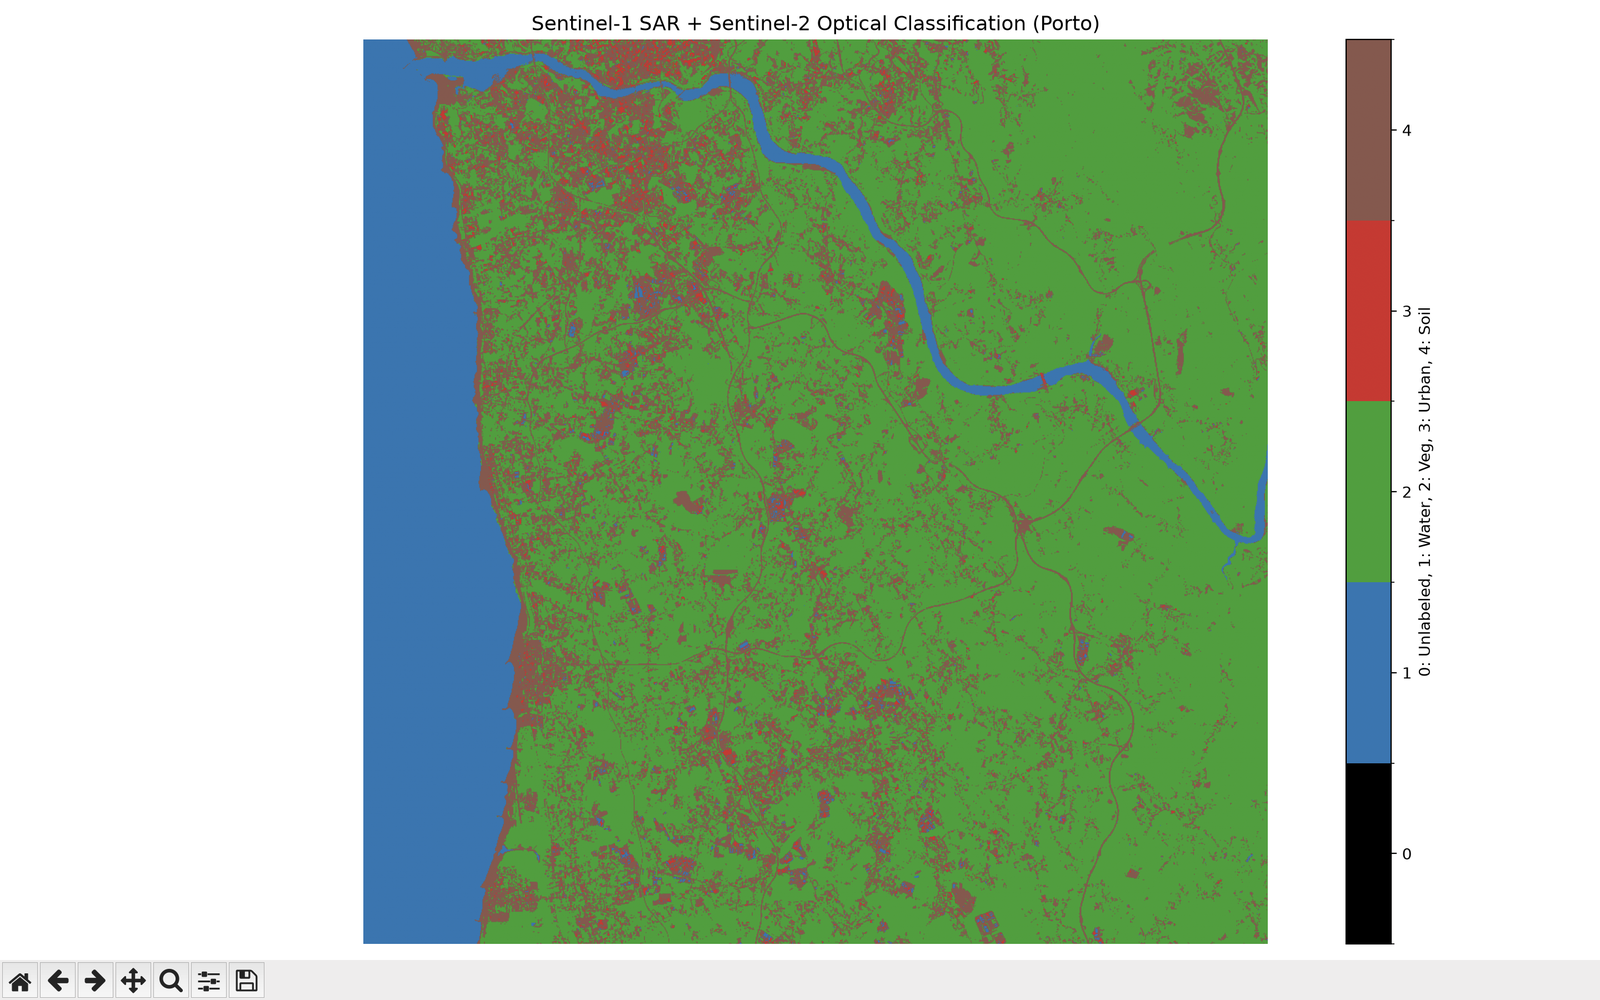
\includegraphics[width=0.78\textwidth]{../outputs/figures/fig_classification.png}
\caption{Random Forest map (Python) from SNAP-collocated S1+S2. Blue: water; green: vegetation; red: urban; brown: bare soil.}
\end{figure}

\begin{figure}[h]
\centering
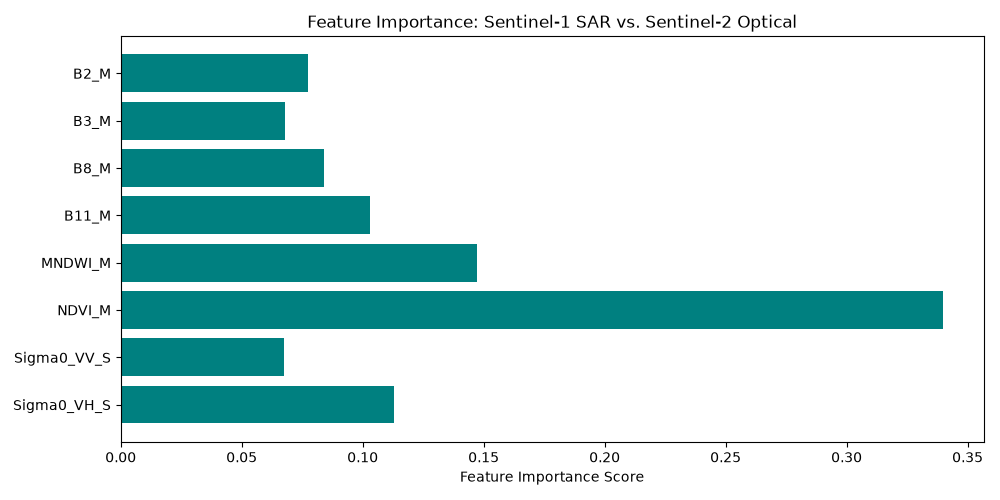
\includegraphics[width=0.72\textwidth]{../outputs/figures/fig_importance.png}
\caption{Feature importance when indices are included as diagnostics. NDVI dominates; $\sigma^0$ VH is the strongest radar contributor.}
\end{figure}

\section{Limitation (the point of this meeting)}
The 100\% figure was a \textbf{data leak}: labels derived from NDVI/MNDWI, then a tree model reproducing that formula, plus neighbouring pixels in both train and test (spatial autocorrelation). Removing indices from training and using block CV is necessary but not sufficient. Independent polygons (hand ROIs, or CORINE / ESA WorldCover) are required before any accuracy is reported as a scientific result.

\section{Proposed next steps (for discussion)}
\begin{enumerate}[leftmargin=1.5em,itemsep=0.15em]
  \item Independent test labels: SNAP/QGIS ROIs versus CORINE or ESA WorldCover.
  \item Add DEM derivatives (slope, aspect) --- Douro valley relief.
  \item Same spatial CV, second classifier (SVM or XGBoost) for a method comparison, not a leaderboard.
\end{enumerate}

\noindent\textbf{Question for the supervisor:} which of (1)--(3) is the right next increment at Erasmus scale?

\vspace{0.6em}
\noindent\textit{I would be grateful for comments on this SNAP--Python workflow, and --- if you are willing to guide the next step --- for a short recommendation letter in due course. I can provide a one-paragraph description of the method and of my own contribution.}

\end{document}
